%!TEX root = thesis.tex
\chapter{Results}\label{chap:results}
\thispagestyle{plain}

% ==== SECTION 1 ===============================================================
\section{Equilibrium experiments} % (fold)
\label{sec:equilibrium_experiments_results}
    Equilibrium experiment are a useful tool to asses the behavior of glacier models. The OGGM provides two climate scenarios for such equilibrium experiments, the \lstinline`ConstantMassBalance` model and the \lstinline`RandomMassBalance` model (see Section~\ref{sub:mass_balance_models_implementation} for implementation details). The experiments are performed on all alpine glaciers using the HISTALP dataset \citep{Auer2007} as climate input data. The baseline climate for each glacier comes from a 31-year period centered around the \textit{equilibrium year} \tstar. An additional temperature bias of \SI{0}{\celsius}, \SI{-0.5}{\celsius} and \SI{+0.5}{\celsius} results in a neutral, positive and negative step change in mass balance, respectively. The detailed experimental setup can be found in Section~\ref{sub:equilibrium_experiments_setup}

    The first qualitative conclusions are drawn from the temporal evolution of length, surface area and ice volume. We are looking at selected single glaciers as well as at the regional scale, i.e. at the sum over all glaciers in the HISTALP domain. Scaling methods applied to a single give only an order of magnitude estimation \citep[section 8.5][cf.]{Bahr2015}, which is accounted for in the following analysis. More quantitative results are drawn from an autocorrelation analysis and a power spectral density analysis, inspired by \citet{Roe2014}.
    
    \subsection{Time series} % (fold)
    \label{sub:time_series_results}

      The following section tries to explain the model behavior using the temporal evolution of the length, surface area and ice volume. The plots show a comparison between the \vas{} model and the flowline model time series, both for the constant and random climate scenario. Since the \vas{} model derives the initial geometry from the surface area, absolute values of initial length and volume differ between the \vas{} model and the flowline model. The results are therefore normalized with respect to their initial values for better comparability. 

      \subsubsection{Hintereisferner test case} % (fold)
      \label{ssub:hintereisferner_test_case_results}

        % Initial paragraph with TL;DR;
        This first test case serves to get Section~\ref{ssub:hintereisferner_test_case_setup}
        The preliminary results 
        All topic are investigated further in the following sections. Following are the preliminary results in accordance to the intended ...
        \begin{enumerate}[label=(\alph*)]
          \item strong underestimation of changes in glacial geometry by the \vas{} model compared to the flowline model
          \item ...
        \end{enumerate}
        Volume, area and length time series are shown in Figure~\ref{fig:hintereisferner}.
        % TODO with a CAPITAL T

        % overall impression, temporal correlation between VAS and flowline
        Both evolution models behave as expected and produce the same qualitative results. The model glacier stays in an approximate equilibrium using the climate around \tstar, decreases ands increases in size for a positive and negative temperature bias of \SI{\pm0.5}{\celsius}. This is true for both mass balance models, whereby the \lstinline`RandomMassBalance` model produces more short term variability (most obviously).
        Glacier advances and retreats correlate nicely between the two evolution models under the same random climatic forcing (with correlation coefficients between 0.44 and 0.72). This is not surprising, given that the implementations of the mass balance models are almost identical. Thereby, the ice volume exhibits the highest year-to-year variability, since volume changes happen instantaneously as function of specific mass balance. The changes in surface area and glacier length are smoother, accounting for the glacier's response time.
        Comparing the evolution models, the flowline model shows stronger long term variations and less short term variability than the \vas{} model. This could indicate higher response times for the flowline model. This assumption is backed by the model behavior under the constant climate scenario. Qualitatively speaking, the flowline model takes longer to reach a new equilibrium (after around 400 years) than the \vas{} model (after around 200 years). A quantitative analysis of the response times follows after the evaluation of the equilibrium values.

        % Equilibrium values
        For the following discussion about the equilibrium values, only the constant climate scenario is considered. It is assumed that the model glacier has reached a new equilibrium after 1'000 years of evolution. Hence, the equilibrium values are taken as the final values at year \lstinline`t = 1000`. This assumption seems valid, given that the values fluctuate only in the order of \SI{0.01}{\percent} over the last 200 years of the simulations.
        The only exception forms the glacier length of the flowline model for with a positive mass balance bias. Under this climate scenario, the equilibrium flowline glacier length oscillates between \SI{9.9}{\kilo\meter} and \SI{10}{\kilo\meter}. The glacier jumps back and for one grid cell, due to the spatial resolution of \SI{100}{\meter} of the flowline model. Hence, the equilibrium length is assumed to be average between both values. Table~\ref{tab:hintereisferner_equilibrium_values} shows all equilibrium values in response to the positive and negative step change in equilibrium climate.

        % Underestimation
        The most apparent result is that the \vas{} model underestimates all changes in glacier geometry when compared to the flowline model. While the \vas{} model predicts a volume change of around \SI{\pm16.5}{\percent}, the flowline ice volume increases by \SI{71}{\percent} and decreases by \SI{42}{\percent}, for the positive and negative mass balance bias, respectively. In other words, the flowline glacier grows more than four times larger and shrinks more than two and a half times smaller than the \vas{} glacier. The surface area is slightly less underestimated, with a change of \SI{\pm12}{\percent} for the \vas{} model versus changes of \SI{+33}{\percent} and \SI{-23}{\percent} for the flowline model. The glacier length of the \vas{} model does hardly change at all. The maximum year-to-year variation under any climate scenario shows slightly more than six meters, which is about \SI{1}{\percent} of the initial value and therefore hardly a physical sensible value. This results in an length change of \SI{\pm7.5}{\percent} for the \vas model, which is roughly five to six times less than the changes of \SI{+44}{\ percent} and \SI{-39}{\percent} for the flowline model. The values proof that the \vas{} model cannot, self-evidently, resolve all processes as dedicated ice physics models can. However, the scaling constant $c$ is a random variable which can vary drastically from glacier to glacier. It is possible that the global mean value of $c=\SI{0.034}{\kilo\meter^{3-2\gamma}}$ is a bad fit for the characteristics of Hintereisferner. A detailed look at the model's sensitivity to the scaling constant is provided in Section~\ref{sub:sensitivity_analysis}.

        % Time scales - segue and introduction
        ... not only the amplitude but also the temporal evolution differs between the two evolution models.

        % Time scales computed by the vas model
        The \vas{} model is implemented with proper response time scaling to estimate temporal changes (see Section~\ref{sub:glacier_evolution_model}). The response time scaling depends on the time scale of the glacier's length change response to volume change $\tau_L$ and the time scale of the glacier's surface area change response to volume change $\tau_A$. The initial time scales computed for the Hintereisferner amount to $\tau_L = \SI{52}{\year}$ and $\tau_L = \SI{52}{\year}$ and 

        % e-folding times

        % Symmetrie
        The changes in glacier geometry produces by the \vas{} model are highly symmetrical for the runs with positive and negative mass balance bias. This can qualitatively seen in Figure~\ref{fig:hintereisferner} and qualitatively in the paragraph above and Table~\ref{tab:hintereisferner_equilibrium_values}. The absolute changes in volume, area and length lie within \SI{1}{\percent} of difference from each other, e.g., volume change of \SI{+17}{\percent} and \SI{-16}{\percent} for a temperature bias of \SI{-0.5}{\celsius} and \SI{+0.5}{\celsius}, respectively.
        % oscialltion
        
        % \begin{table}[htp]
        %   \centering
        %   \ra{1.4}
        %   \caption{Hintereisferner (RGI60-11.00897) equilibrium values after 1000 years of model evolution under a constant equilibrium climate with a temperature bias of \SI{-0.5}{\celsius} and \SI{+0.5}{\celsius}, respectively. Percentage values in parenthesis indicate normalized values in respective to their initial values.}
        %   \label{tab:hintereisferner_equilibrium_values}
        %   \begin{tabular}{@{}lrlcrlcrlcrl@{}}
        %     \toprule
        %     {} & \multicolumn{5}{c}{$\bm{\Delta T}$\textbf{ = \SI{-0.5}{\celsius}}} & \phantom{a} & \multicolumn{5}{c}{$\bm{\Delta T}$\textbf{ = \SI{+0.5}{\celsius}}} \\
        %     \cmidrule{2-6} \cmidrule{8-12}

        %     {} & \multicolumn{2}{c}{V/A scaling} & \phantom {} & \multicolumn{2}{c}{Flowline} & \phantom{a} & \multicolumn{2}{c}{V/A scaling} & \phantom {} & \multicolumn{2}{c}{Flowline} \\
        %     \midrule
        %     \textbf{Volume [\si{\cubic\kilo\meter}]} &  0.70 & (117\%) & \phantom {} &  1.37 & (171\%) & \phantom{a} &  0.50 & (84\%) & \phantom {} &  0.47 & (58\%) \\
        %     \textbf{Area [\si{\square\kilo\meter}]} &  9.02 & (112\%) & \phantom {} &  10.68 & (133\%) & \phantom{a} &  7.08 & (88\%) & \phantom {} &  6.17 & (77\%) \\
        %     \textbf{Length [\si{\kilo\meter}]} &  5.26 & (107\%) & \phantom {} &  9.95 & (144\%) & \phantom{a} &  4.52 & (92\%) & \phantom {} &  4.20 & (61\%) \\
        %     \bottomrule
        %   \end{tabular}
        % \end{table}

        \begin{sidewaystable}[htp]
          \centering
          \ra{1.4}
          \caption{Hintereisferner (RGI60-11.00897) equilibrium values after 1000 years of model evolution under a constant equilibrium climate with a temperature bias of \SI{-0.5}{\celsius} and \SI{+0.5}{\celsius}, respectively. Percentage values in parenthesis indicate normalized values in respective to their initial values.}
          \label{tab:hintereisferner_equilibrium_values}
          \begin{tabular}{@{}lcccrlcrlcrlcrl@{}}
            \toprule
            % first level header
            {} & \multicolumn{2}{c}{\textbf{Initial values}} & \phantom{asdf} & \multicolumn{5}{c}{$\bm{\Delta T}$\textbf{ = \SI{-0.5}{\celsius}}} & \phantom{a} & \multicolumn{5}{c}{$\bm{\Delta T}$\textbf{ = \SI{+0.5}{\celsius}}} \\
            % second level header
            \cmidrule{2-3} \cmidrule{5-9} \cmidrule{11-15}
            {} & V/A scaling & Flowline & \phantom {} & \multicolumn{2}{c}{V/A scaling} & \phantom {} & \multicolumn{2}{c}{Flowline} & \phantom{a} & \multicolumn{2}{c}{V/A scaling} & \phantom {} & \multicolumn{2}{c}{Flowline} \\
            % table body
            % volume
            \midrule
            \textbf{Volume [\si{\cubic\kilo\meter}]} & 0.60 & 0.80 & &  0.70 & (117\%) & \phantom {} &  1.37 & (171\%) & \phantom{a} &  0.50 & (84\%) & \phantom {} &  0.47 & (58\%) \\
            % area
            \textbf{Area [\si{\square\kilo\meter}]} & 8.04 & 8.04 & &  9.02 & (112\%) & \phantom {} &  10.68 & (133\%) & \phantom{a} &  7.08 & (88\%) & \phantom {} &  6.17 & (77\%) \\
            % length
            \textbf{Length [\si{\kilo\meter}]} & 4.89 & 6.90 & & 5.26 & (107\%) & \phantom {} &  9.95 & (144\%) & \phantom{a} &  4.52 & (92\%) & \phantom {} &  4.20 & (61\%) \\
            \bottomrule
          \end{tabular}
        \end{sidewaystable}

        \begin{table}[htp]
          \centering
          \small
          \ra{1.4}
          \caption{Hintereisferner (RGI60-11.00897) equilibrium values after 1000 years of model evolution under a constant equilibrium climate with a temperature bias of \SI{-0.5}{\celsius} and \SI{+0.5}{\celsius}, respectively. Percentage values in parenthesis indicate normalized values in respective to their initial values.}
          \label{tab:hintereisferner_equilibrium_values}
          \begin{tabular}{@{}rcrlcrlcrl@{}}
            \toprule
            {} & \phantom{a} & \multicolumn{2}{c}{\textbf{Length [\si{\kilo\meter}]}} & \phantom{a} & \multicolumn{2}{c}{\textbf{Area [\si{\square\kilo\meter}]}} & \phantom{a} & \multicolumn{2}{c}{\textbf{Volume [\si{\cubic\kilo\meter}]}} \\
            \midrule
            \textbf{Initial values} \\
            V/A scaling & \phantom{a} & 4.89 & (1.00) & \phantom{a} & 8.04 & (1.00) & \phantom{a} & 0.60 & (1.00) \\
            Flowline & \phantom{a} &  6.90 & (1.00) & \phantom{a} & 8.04 & (1.00) & \phantom{a} & 0.80 & (1.00) \\
            $\bm{\Delta T}$\textbf{ = \SI{-0.5}{\celsius}} \\
            % \cmidrule{1-10}
            V/A scaling & \phantom{a} & 5.26 & (1.07) & \phantom{a} & 9.02 & (1.12) & \phantom{a} & 0.70 & (1.17) \\
            Flowline & \phantom{a} &  9.95 & (1.44) & \phantom{a} & 10.68 & (1.33) & \phantom{a} &  1.37 & (1.71) \\
            \addlinespace
            $\bm{\Delta T}$\textbf{ = \SI{+0.5}{\celsius}} \\
            % \cmidrule{1-10}
            V/A scaling & \phantom{a} & 4.52 & (0.92) & \phantom{a} & 7.08 & (0.88) & \phantom{a} & 0.50 & (0.84) \\
            Flowline & \phantom{a} &   4.20 & (0.61) & \phantom{a} & 6.17 & (0.77) & \phantom{a} & 0.47 & (0.58) \\
            \bottomrule
          \end{tabular}
        \end{table}
        
        % Text with all the equilibrium values contained in the table, don't know if to inlcude since it looks/reads weird.
        % The equilibrium ice volume for the positive and negative mass balance scenario is \SI{0.70}{\cubic\kilo\meter} (\SI{117}{\percent}) and \SI{0.50}{\cubic\kilo\meter} (\SI{84}{\percent}) for the \vas{} model and \SI{1.37}{\cubic\kilo\meter} (\SI{171}{\percent}) and \SI{0.47}{\cubic\kilo\meter} (\SI{58}{\percent}) for the flowline model, respectively. The values in parenthesis are normalized with the respective initial values. The equilibrium surface area for the positive and negative mass balance scenario is \SI{9.02}{\squared\kilo\meter} (\SI{112}{\percent}) and \SI{7.08}{\squared\kilo\meter} (\SI{88}{\percent}) for the \vas{} model and \SI{10.68}{\squared\kilo\meter} (\SI{133}{\percent}) and \SI{6.17}{\squared\kilo\meter} (\SI{77}{\percent}) for the flowline model, respectively. The equilibrium length for the positive and negative mass balance scenario is \SI{5.26}{\kilo\meter} (\SI{107}{\percent}) and \SI{4.52}{\kilo\meter} (\SI{92}{\percent}) for the \vas{} model and \SI{9.95}{\kilo\meter} (\SI{144}{\percent}) and \SI{4.20}{\kilo\meter} (\SI{61}{\percent}) for the flowline model, respectively.

        % Response time and oscillating behavior

        \begin{figure}[htp]
          \centering
          % VAS volume
          \begin{subfigure}[b]{0.476\textwidth}
            \caption{\Vas{} model, relative ice volume}
            \label{fig:hintereisferner:volume_vas}
            \centering
            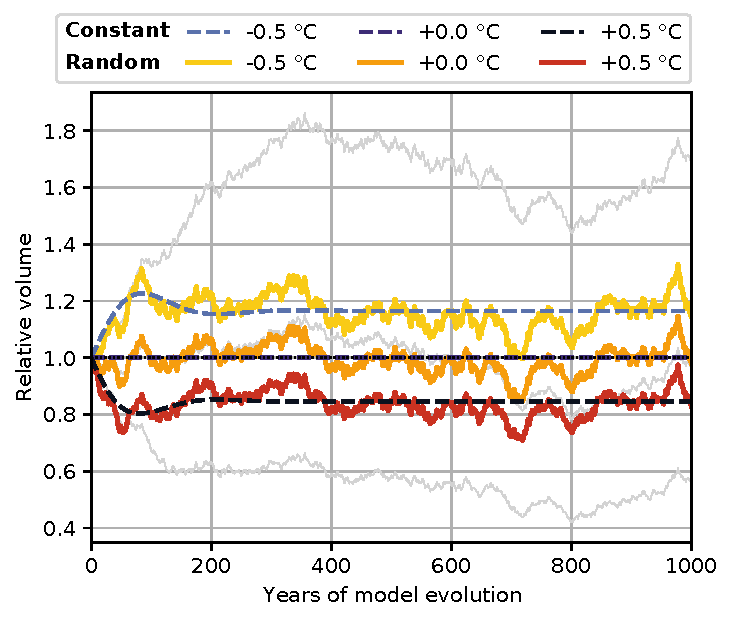
\includegraphics[width=\textwidth]{../plots/final_plots/time_series/single_glaciers/volume_norm_vas_Hintereisferner.pdf}
          \end{subfigure}
          \hfill
          % Flowline volume
          \begin{subfigure}[b]{0.476\textwidth}
            \caption{Flowline model, relative ice volume}
            \label{fig:hintereisferner:volume_fl}
            \centering
            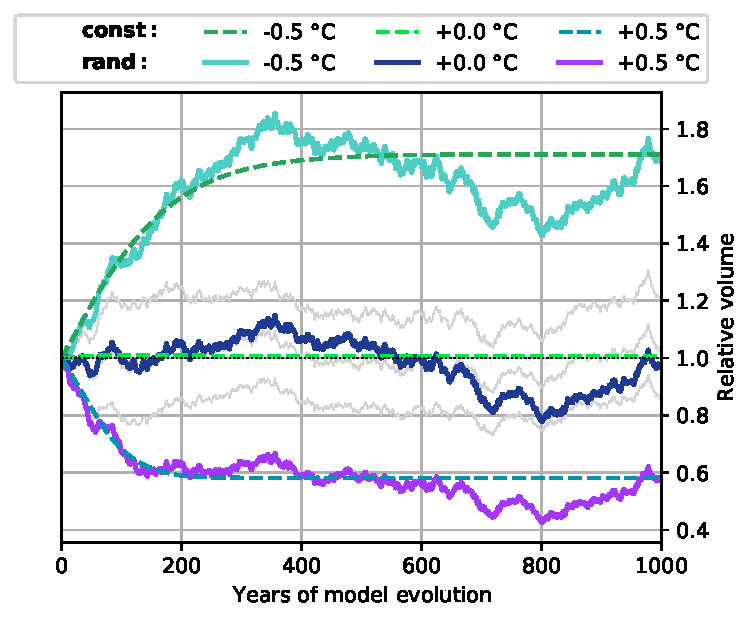
\includegraphics[width=\textwidth]{../plots/final_plots/time_series/single_glaciers/volume_norm_fl_Hintereisferner.pdf}
          \end{subfigure}
          % VAS area
          \begin{subfigure}[b]{0.476\textwidth}
            \caption{\Vas{} model, relative surface area}
            \label{fig:hintereisferner:area_vas}
            \centering
            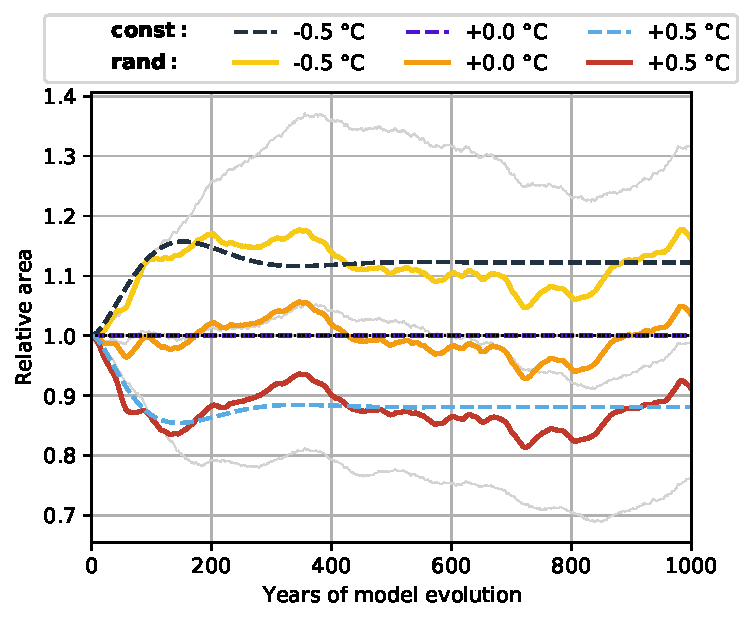
\includegraphics[width=\textwidth]{../plots/final_plots/time_series/single_glaciers/area_norm_vas_Hintereisferner.pdf}
          \end{subfigure}
          \hfill
          % Flowline area
          \begin{subfigure}[b]{0.476\textwidth}
            \caption{Flowline model, relative surface area}
            \label{fig:hintereisferner:area_fl}
            \centering
            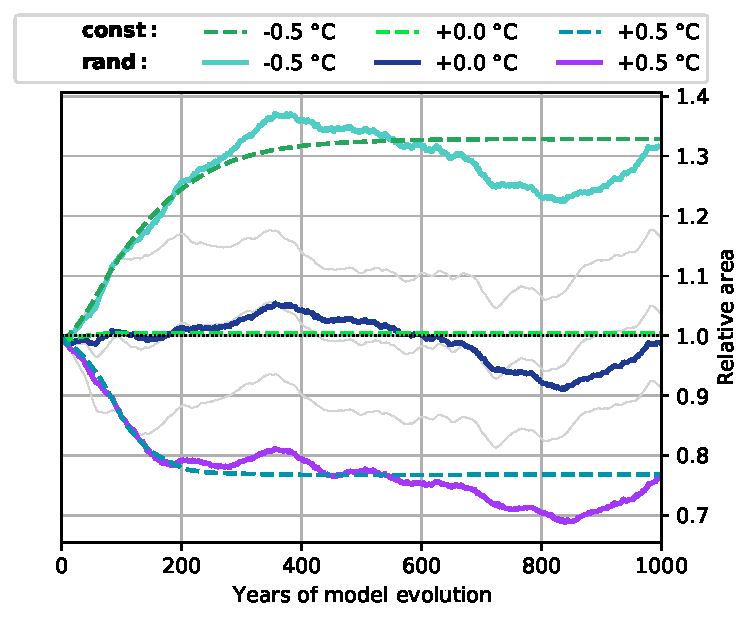
\includegraphics[width=\textwidth]{../plots/final_plots/time_series/single_glaciers/area_norm_fl_Hintereisferner.pdf}
          \end{subfigure}
          % VAS length
          \begin{subfigure}[b]{0.476\textwidth}
            \caption{\Vas{} model, relative glacier length}
            \label{fig:hintereisferner:length_vas}
            \centering
            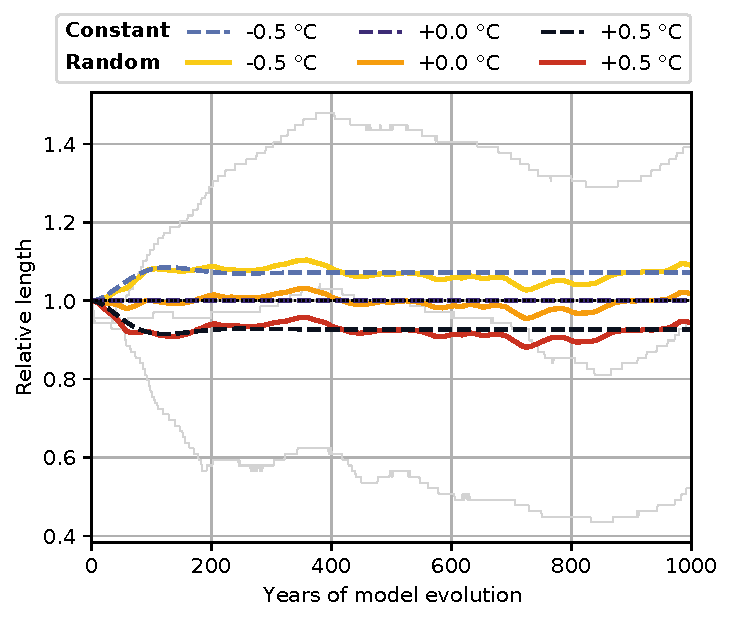
\includegraphics[width=\textwidth]{../plots/final_plots/time_series/single_glaciers/length_norm_vas_Hintereisferner.pdf}
          \end{subfigure}
          \hfill
          % Flowline length
          \begin{subfigure}[b]{0.476\textwidth}
            \caption{Flowline model, relative glacier length}
            \label{fig:hintereisferner:length_fl}
            \centering
            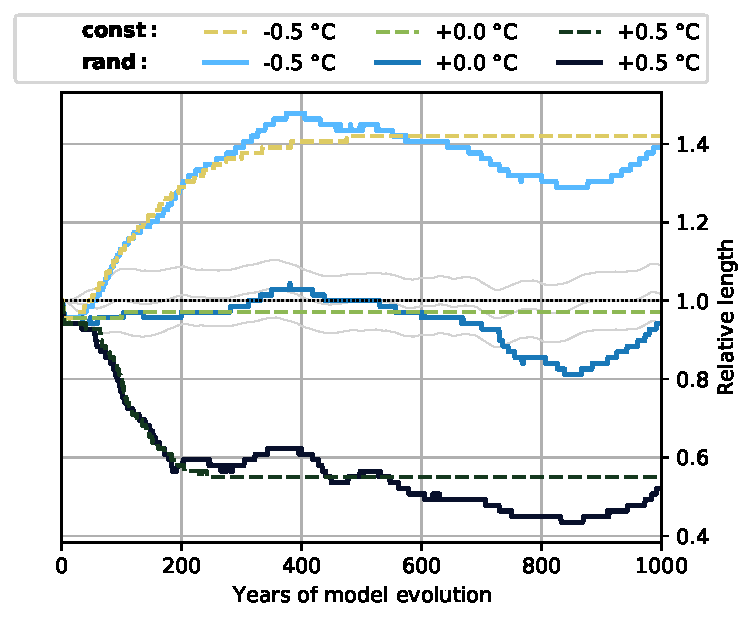
\includegraphics[width=\textwidth]{../plots/final_plots/time_series/single_glaciers/length_norm_fl_Hintereisferner.pdf}
          \end{subfigure}
          
          \caption{Temporal evolution of ice volume in (\subref{fig:hintereisferner:volume_vas}) and (\subref{fig:hintereisferner:volume_fl}), surface area in (\subref{fig:hintereisferner:area_vas}) and (\subref{fig:hintereisferner:area_fl}) and glacier length in (\subref{fig:hintereisferner:length_vas}) and (\subref{fig:hintereisferner:length_fl}) for Hintereisferner (RGI60-11.00897). The shown values area normalized with their respective initial values. The left panels show the result of the \vas{} model, the right panels show the results of the flowline model. Solid lines represent the random climate scenarios, while dashed lines represent the constant climate scenarios. All climate scenarios are based on an equilibrium climate. The applied temperature biases of \SI{-.5}{\celsius}, \SI{0}{\celsius} and \SI{+.5}{\celsius} are color coded, see legend for details. The dotted line indicates the initial volume. The light gray lines represent the volume evolutions of the other model, to facilitate comparisons.}
          \label{fig:hintereisferner}
        \end{figure}
      
      % subsubsection hintereisferner_test_case_results (end)

      \subsubsection*{Overall findings}

      \begin{itemize}
        \item 
        \item The size (length, area, volume) changes drastically less (i.e., between two to eight times less) with the \vas{} model than with the flowline model.
        However, volume estimations from volume/area scaling of a single glaciers must be considered as order of magnitude result. The scaling constant $c$ is a random variable which can vary drastically from to glacier. Apparently, the global mean value of $c=0.034\ \mathrm{km^{3-2\gamma}}$ is a bad fit for the characteristics of Hintereisferner.
      \end{itemize}
      

      1. 

      2. The size changes (dramatically) less under the VAS model than under the flowline model (true for length, area, and volume).

         *Note*: However, volume estimations from volume/area scaling of a single glaciers must be considered as order of magnitude result. The scaling constant $c$ is a random variable which varies (drastically) from to glacier. Apparently, the global mean value of $c=0.034\ \mathrm{km^{3-2\gamma}}$ is a bad fit for the characteristics of Hintereisferner.

         *Second Note*: Changing the scaling constants changes the absolute values of ice volume (as well as surface area and length). A higher volume/area scaling constant results in a larger initial ice volume. Subjected to the same climate perturbation (temperature step change), an initially larger will gain/loose more ice and reach a higher equilibrium ice volume than a smaller one. However, when normalized with initial ice volume there are no more discernible differences in the magnitude of ice volume change. The temporal evolution, i.e., the oscillation behavior, is comparable, even if smaller glaciers react faster than larger ones (which is to be expected).

         *TL;DR; Turns out, the scaling constant does not change the magnitude of the normalized volume change.* 

      3. The length of the VAS model has to be seen more as a model parameter, rather than as an actual property. The VAS length decreases/increases only by about 8 percent compared to its initial value, for a positive/negative temperature bias of 0.5 °C. This correspond to an absolute length change of less than 400 m, which is very little compared to the 3 to 4 km in length change (~40% of the initial value) produced by the flowline model. (*Note*: May change with different $c$ parameter. *Second note*: Turns out, it does not when normalized with initial length.)

      4. The result of VAS model under a constant climate scenario with a non-zero temperature bias reminds of a damped oscillating signal. The modeled length reaches its maximum after ~200 years, overshooting the equilibrium result by more than 1%. Followed by two minor but still discernible peaks until the new equilibrium is reached. Both, surface area and volume reach their maximum earlier and overshoot by more.

      \subsubsection{Commitment runs} % (fold)
      \label{ssub:commitment_runs_results}

        The findings explained hereafter result from runs under
        \begin{enumerate*}[label=(\alph*)]
          \item equilibrium climate, with \lstinline`y0` = \tstar{} for each glacier
          \item todays climate, with \lstinline`y0 = 1999`
        \end{enumerate*}.
        Both climate scenarios run with different mass balance model and apply different temperature biases. For more details see Section~\ref{ssub:commitment_runs_setup}.

        Let's first take a more general look at the model behavior under equilibrium climate. Both evolution models run for 1'000 years, once with the \lstinline`ConstantMassBalance` model and once with the \lstinline`RandomMassBalance` model. A random climate with its year-to-year fluctuations is obviously more physical than a completely constant climate. However, the changes in glacier ice volume under both climate scenarios are almost identical. Over the last 200 years of the simulations with equilibrium climate, the differences in total ice volume between the constant and random climate scenario average around \SI{0.6}{\percent} to \SI{0.7}{\percent} for the \vas{} model and \SI{0.7}{\percent} to \SI{2.3}{\percent} for the flowline model, depending on the temperature bias. This makes intuitive sense, considering that glaciers act as natural low-pass filters for climatic variabilities. For simplicity, all following values correspond to the results under a constant climate scenario.

      

        The \vas{} model estimates a total ice volume of \SI{139}{\cubic\kilo\meter} (\SI{106}{\percent}), \SI{115}{\cubic\kilo\meter} (\SI{88}{\percent}) and \SI{95}{\cubic\kilo\meter} (\SI{73}{\percent}), for a temperature bias of \SI{-.5}{\celsius}, \SI{0}{\celsius} and \SI{+.5}{\celsius}, respectively. The flowline model estimates a total ice volume of \SI{236}{\cubic\kilo\meter} (\SI{145}{\percent}), \SI{147}{\cubic\kilo\meter} (\SI{90}{\percent}) and \SI{86}{\cubic\kilo\meter} (\SI{53}{\percent}), for a temperature bias of \SI{-.5}{\celsius}, \SI{0}{\celsius} and \SI{+.5}{\celsius}, respectively.
        Both evolution models adjust their initial ice volume downwards by \SI{12}{\percent} (\vas) and \SI{10}{\percent} (flowline) under equilibrium climate. This is due to the mass balance residual \bias{}. It indicates that the 2003 ge
        As seen before, the \vas{} scaling model underestimates the change in ice volume compared to the flowline model. 

        \begin{figure}[htp]
          \centering
          \begin{subfigure}[b]{0.48\textwidth}
            \caption{\Vas{} model, relative glacier volume}
            \label{fig:histalp_commitment:volume_norm_const}
            \centering
            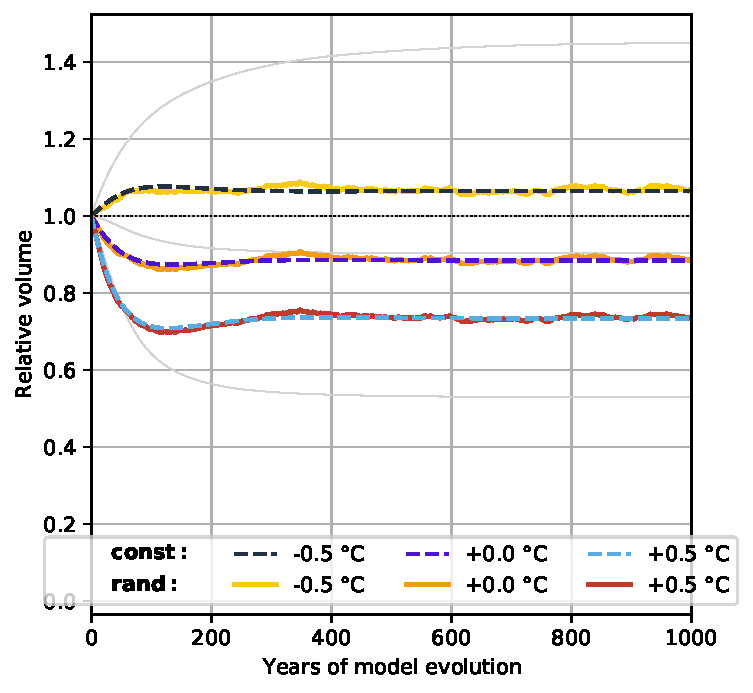
\includegraphics[width=\textwidth]{../plots/final_plots/time_series/histalp_commitment/volume_norm_vas.pdf}
          \end{subfigure}
          \hfill
          \begin{subfigure}[b]{0.48\textwidth}
            \caption{Flowline model, relative glacier volume}
            \label{fig:histalp_commitment:volume_norm_random}
            \centering
            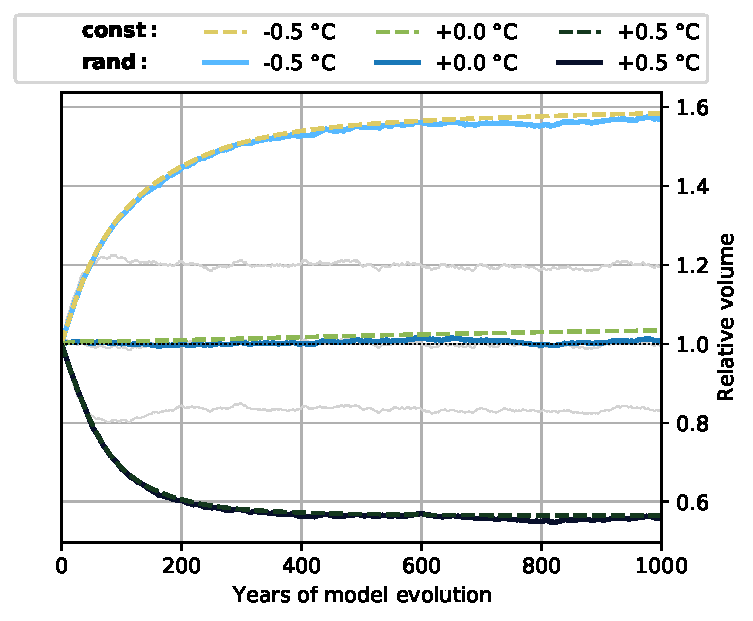
\includegraphics[width=\textwidth]{../plots/final_plots/time_series/histalp_commitment/volume_norm_fl.pdf}
          \end{subfigure}
          \begin{subfigure}[b]{0.48\textwidth}
            \caption{\Vas{} model, absolute glacier volume}
            \label{fig:histalp_commitment:volume_abs_const}
            \centering
            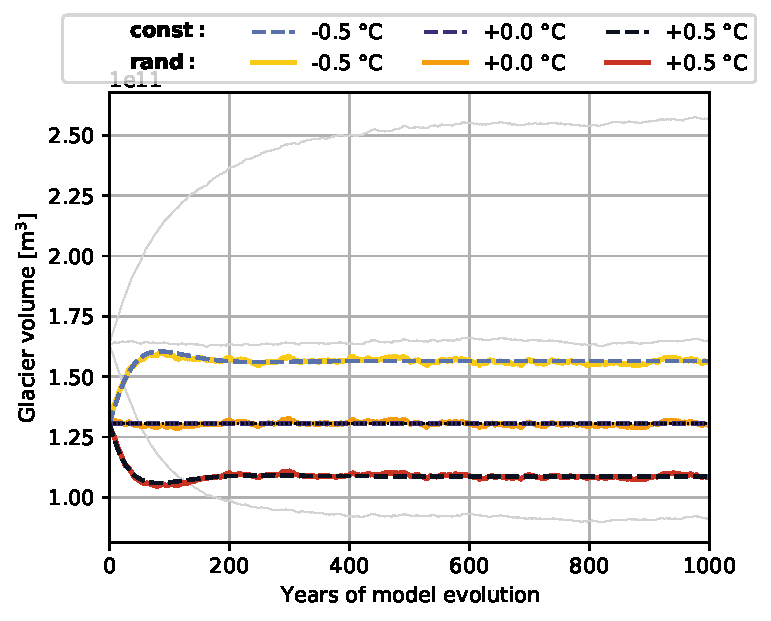
\includegraphics[width=\textwidth]{../plots/final_plots/time_series/histalp_commitment/volume_abs_vas.pdf}
          \end{subfigure}
          \hfill
          \begin{subfigure}[b]{0.48\textwidth}
            \caption{Flowline model, absolute glacier volume}
            \label{fig:histalp_commitment:volume_abs_random}
            \centering
            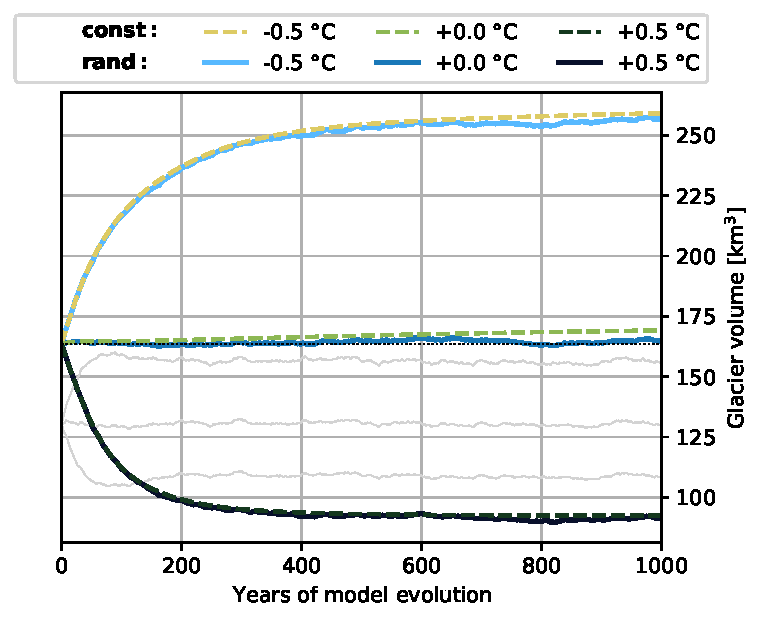
\includegraphics[width=\textwidth]{../plots/final_plots/time_series/histalp_commitment/volume_abs_fl.pdf}
          \end{subfigure}
          
          \caption{Time series of total ice volume for all glaciers in the HISTALP domain. The upper two panels show the relative glacier ice volume, normalized with the initial values, while the lower two panels show the absolute glacier ice volume. The left panels show the result of the \vas{} model, the right panels show the results of the flowline model. Solid lines represent the random climate scenarios, while dashed lines represent the constant climate scenarios. All climate scenarios are based on an equilibrium climate, with one of three different temperature biases.
          Yellow, orange and red solid lines represent the \vas{} model, while cyan, blue and purple solid lines represent the flowline model, under a random climate with a temperature bias of \SI{-.5}{\celsius}, \SI{0}{\celsius} and \SI{+.5}{\celsius}, respectively. Yellow, orange and red dashed lines represent the \vas{} model, while cyan, blue and purple dashed lines represent the flowline model, under a constant climate with a temperature bias of \SI{-.5}{\celsius}, \SI{0}{\celsius} and \SI{+.5}{\celsius}, respectively. %TODO change colors
          The dotted line indicate the initial volume. The light gray lines represent the volume evolutions of the other model, to facilitate comparisons.}
          \label{fig:histalp_commitment}
        \end{figure}

        % \begin{figure}[htp]
        %   \centering
        %   \begin{subfigure}[b]{0.99\textwidth}
        %     \caption{Normalized glacier volume}
        %     \label{fig:histalp_commitment:volume_norm}
        %     \centering
        %     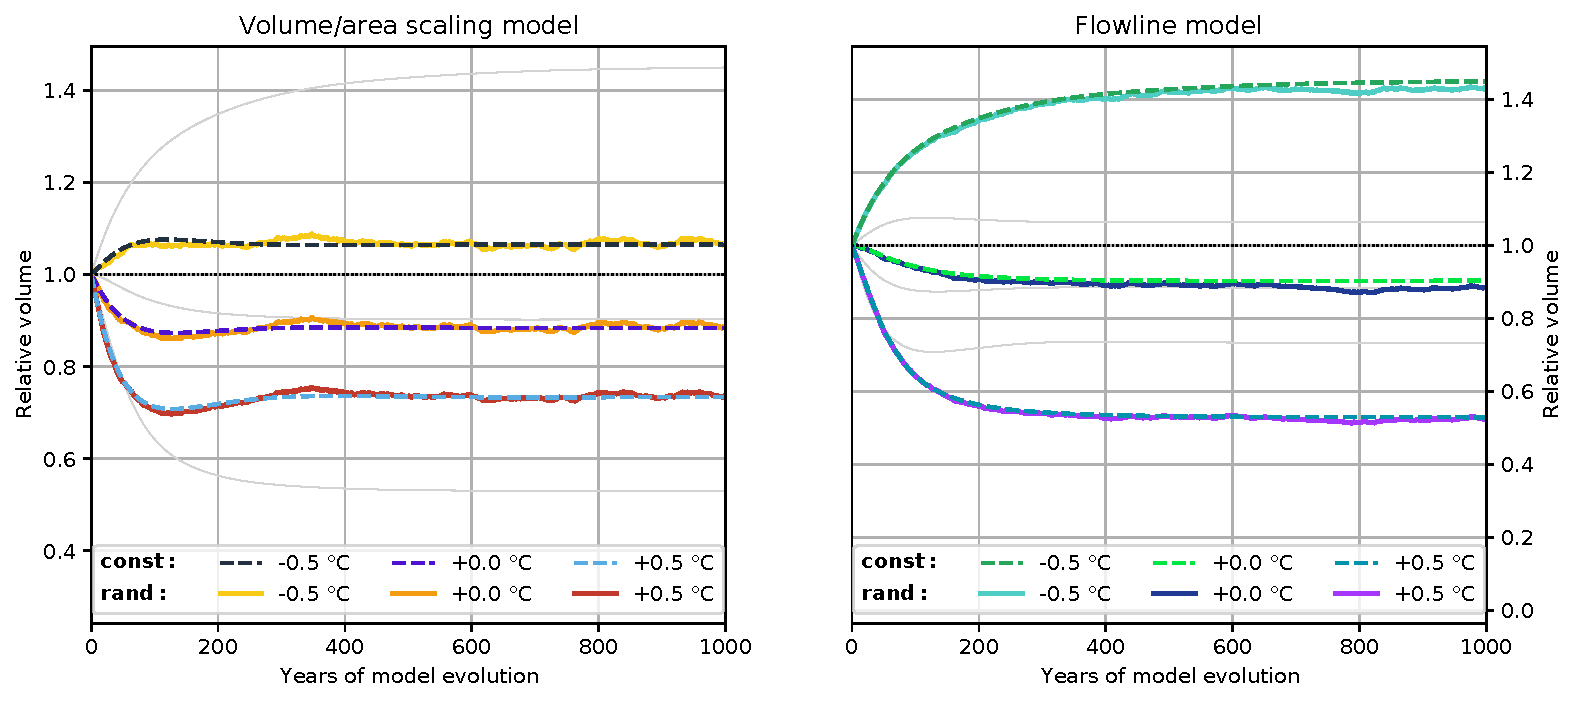
\includegraphics[width=\textwidth]{../plots/final_plots/time_series/histalp_commitment/volume_norm.pdf}
        %   \end{subfigure}
        %   \begin{subfigure}[b]{0.99\textwidth}
        %     \caption{Absolute glacier volume}
        %     \label{fig:histalp_commitment:volume_abs}
        %     \centering
        %     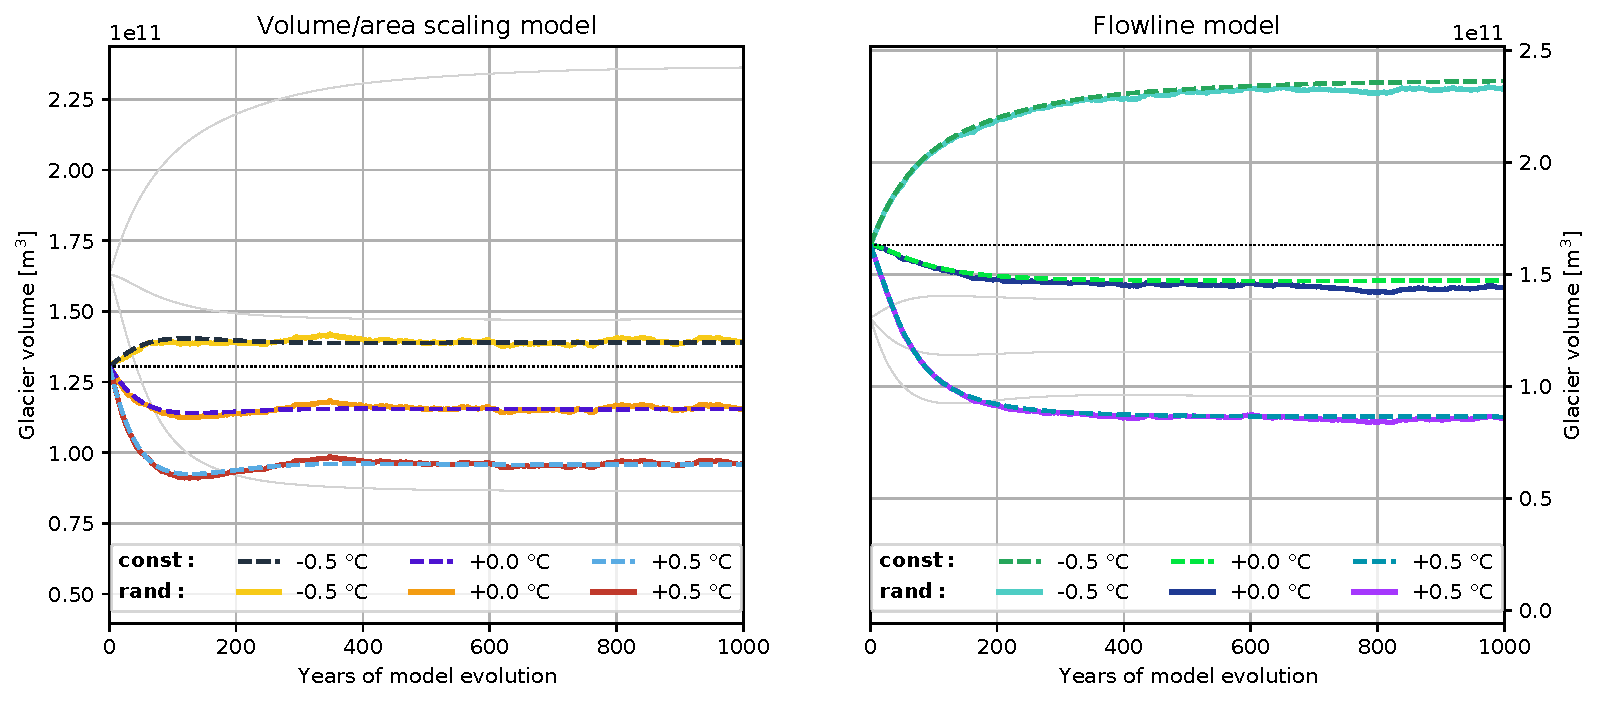
\includegraphics[width=\textwidth]{../plots/final_plots/time_series/histalp_commitment/volume_abs.pdf}
        %   \end{subfigure}
          
        %   \caption{Time series of total ice volume for all glaciers in the HISTALP domain. The upper two panels show the relative values, normalized with the initial values, while the lower two panels show absolute values. The left panels show the result of the \vas{} model, the right panels show the results of the flowline model. Solid lines represent a random climate scenario, while dashed lines represent a constant climate scenario. All climate scenarios are based on an equilibrium climate, however with three different temperature biases.
        %   Yellow, orange and red solid lines represent the \vas{} model, while cyan, blue and purple solid lines represent the flowline model, under a random climate with a temperature bias of \SI{-.5}{\celsius}, \SI{0}{\celsius} and \SI{+.5}{\celsius}, respectively. Yellow, orange and red dashed lines represent the \vas{} model, while cyan, blue and purple dashed lines represent the flowline model, under a constant climate with a temperature bias of \SI{-.5}{\celsius}, \SI{0}{\celsius} and \SI{+.5}{\celsius}, respectively. %TODO change colors
        %   The dotted line indicate the initial volume. The light gray lines represent the volume evolutions of the other model, to facilitate comparisons.}
        %   \label{fig:histalp_commitment}
        % \end{figure}

      
      % subsubsection commitment_runs_results (end)

    % subsection time_series (end)

    \subsection{Autocorrelation analysis} % (fold)
    \label{sub:autocorrelation_analysis_results}

      The autocorrelation function for selected glaciers is shown in Figure~\ref{fig:acf}. For details about the experimental setup see Section~\ref{ssub:autocorrelation_analysis_setup}

      The autocorrelation function of the \vas{} length shows little to no variability between runs under different climate conditions. % TODO compare with almost linear behavior of mass balance model in the vicinity of equilibirum
      The autocorrelation function of the \vas{} length is comparable even between different glaciers. It has the same behavior of a dampened oscillator as described above. Their are differences in amplitude and frequency--most likely affected by size--the general behavior is almost identical. 
      
      The flowline model is able to represent different glacial geometries and grasp individual responses to climatic forcings, which can be seen in the vastly different autocorrelation functions. They differ from to glacier, but also for different climate scenarios (temperature biases) on the same glacier. However, there are no discernible patterns, which again confirms the notion that the OGGM flowline model is capable of modeling each glaciers individual response. Here are some examples: for Hintereisferner the autocorrelation of the flowline model is stronger than that of the \vas{} model, while for Mer de Glace and Großer Aletschgletscher it is lower (for all tested climate scenarios); the flowline model of the Pasterze shows a strong autocorrelation under the equilibrium climate, i.e., \SI{0}{\celsius} temperature bias, (>0.7 for lags times between 0 and 95 years, still >0.43 for 200 years lag time, statistically significant up until a lag time of 232 years), while with a positive and negative temperature bias of \SI{\pm0.5}{\celsius} the autocorrelation is less than for the \vas{} model.
      The \vas{} model has a stronger autocorrelation for short lag time (i.e., less than about 20 years) than the flowline model; similarly, the flowline model of the d'Argentière shows a strong autocorrelation under the climate with \SI{+0.5}{\celsius} temperature bias, and lower autocorrelation than the \vas{} model for the other two climate scenarios; The only observation made for all glaciers, it that the \vas{} model has a stronger autocorrelation for short lag time (i.e., less than about 20 years) than the flowline model. This is true even for glaciers, where the autocorrelation of the flowline mode is generally stronger (e.g., Hintereisferner). 

      It is not the intent of this work to investigate the relation between a glacier's geometry and its autocorrelation function, therefore we leave it at this qualitative first look. However, it is notable that the OGGM flowline model behaves differently for different glaciers and/or different climatic forcings. How far these results are comparable to real world glaciers is anyones guess. The \textit{one size fits all} approach of the \vas{} model produces comparable results, mostly independent the glaciers geometry and the climate forcing (which was to be expected).


      \begin{figure}[htp]
        \centering
        \begin{subfigure}[b]{0.48\textwidth}
          \caption{RGI60-11.00897 - Hintereisferner}
          \label{fig:acf:hintereisferner}
          \centering
          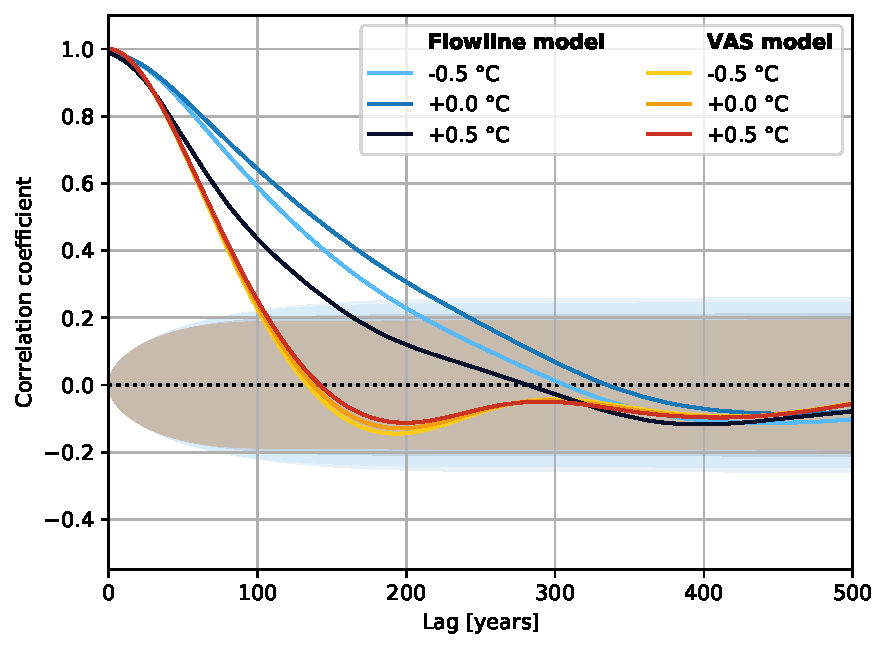
\includegraphics[width=\textwidth]{../plots/final_plots/acf/Hintereisferner.pdf}
        \end{subfigure}
        \hfill
        \begin{subfigure}[b]{0.48\textwidth}
          \caption{RGI60-11.00106 - Pasterze}
          \label{fig:acf:pasterze}
          \centering
          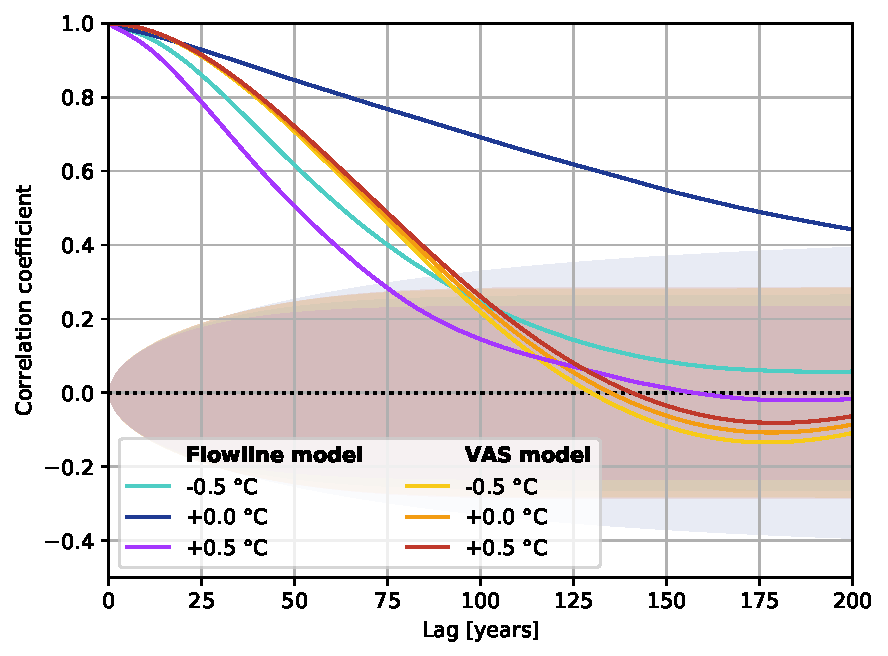
\includegraphics[width=\textwidth]{../plots/final_plots/acf/Pasterze.pdf}
        \end{subfigure}
        \begin{subfigure}[b]{0.48\textwidth}
          \caption{RGI60-11.03643 - Mer de Glace}
          \label{fig:acf:mer_de_glace}
          \centering
          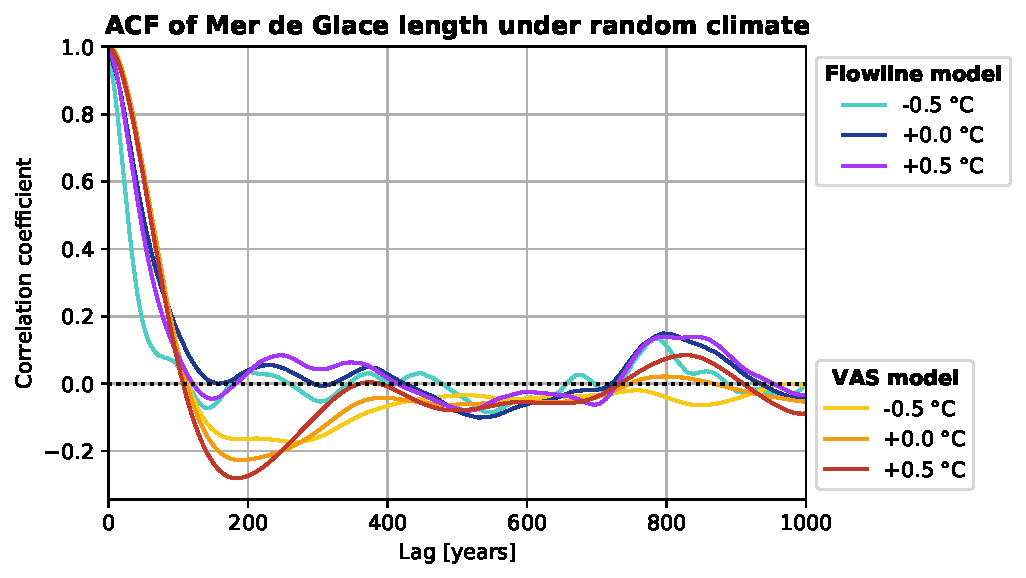
\includegraphics[width=\textwidth]{../plots/final_plots/acf/Mer_de_Glace.pdf}
        \end{subfigure}
        \hfill
        \begin{subfigure}[b]{0.48\textwidth}
          \caption{RGI60-11.03638 - d'Argentière}
          \label{fig:acf:glacier_d_argentiere}
          \centering
          \includegraphics[width=\textwidth]{../plots/final_plots/acf/Glacier_d'Argentière.pdf}
        \end{subfigure}
        \begin{subfigure}[b]{0.48\textwidth}
          \caption{RGI60-11.01450 - Großer Aletschgletscher}
          \label{fig:acf:großer_aletschgletscher}
          \centering
          \includegraphics[width=\textwidth]{../plots/final_plots/acf/Großer_Aletschgletscher.pdf}
        \end{subfigure}
        \hfill
        \begin{subfigure}[b]{0.48\textwidth}
          \caption{RGI60-11.01238 - Rhonegletscher}
          \label{fig:acf:rhonegletscher}
          \centering
          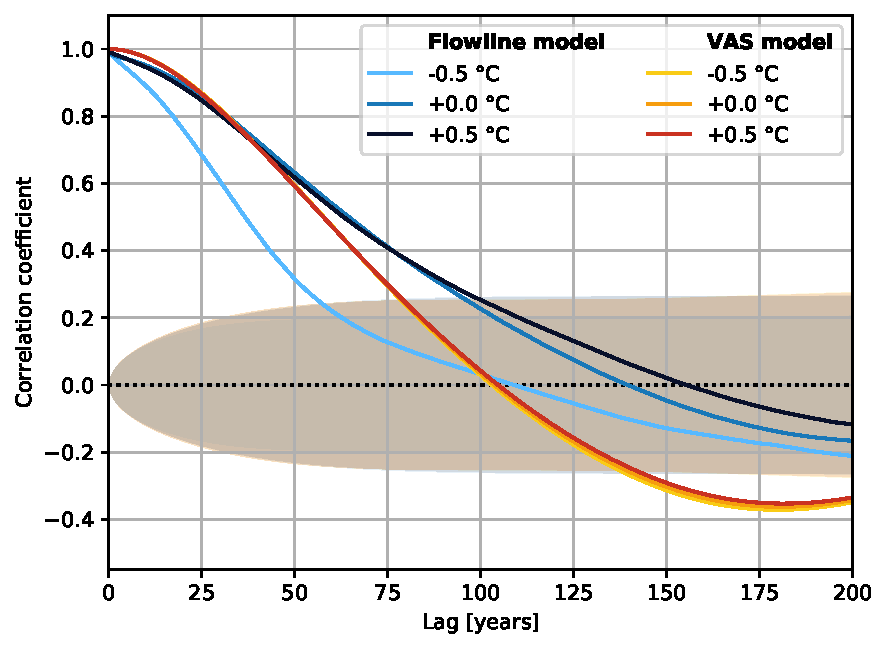
\includegraphics[width=\textwidth]{../plots/final_plots/acf/Rhonegletscher.pdf}
        \end{subfigure}
        % \begin{subfigure}[b]{0.48\textwidth}
        %   \caption{RGI60-11.02704 - Allalingletscher}
        %   \label{fig:acf:allalingletscher}
        %   \centering
        %   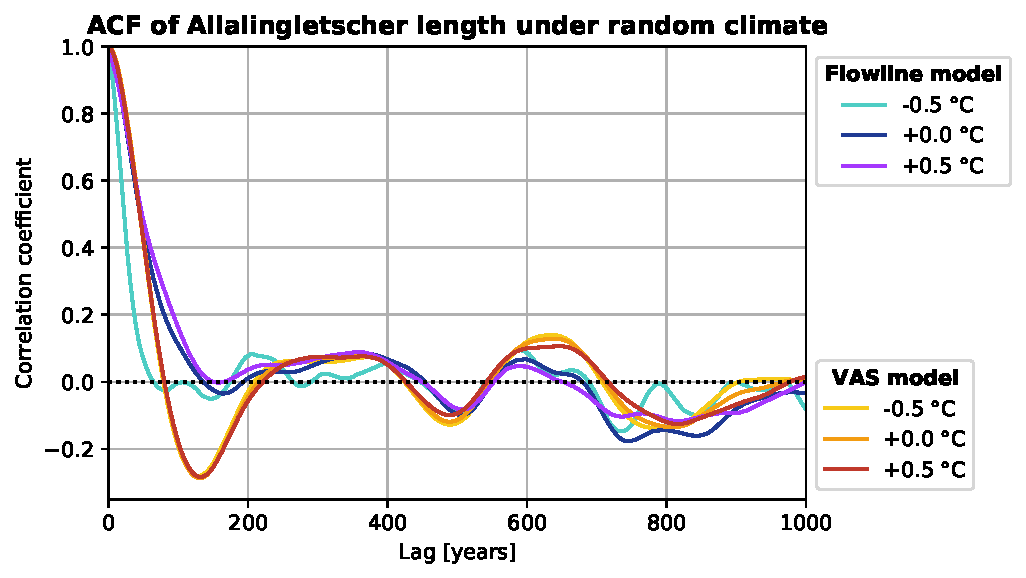
\includegraphics[width=\textwidth]{../plots/final_plots/acf/Allalingletscher.pdf}
        % \end{subfigure}
        % \hfill
        % \begin{subfigure}[b]{0.48\textwidth}
        %   \caption{RGI60-11.02773 - Findelgletscher}
        %   \label{fig:acf:findelgletscher}
        %   \centering
        %   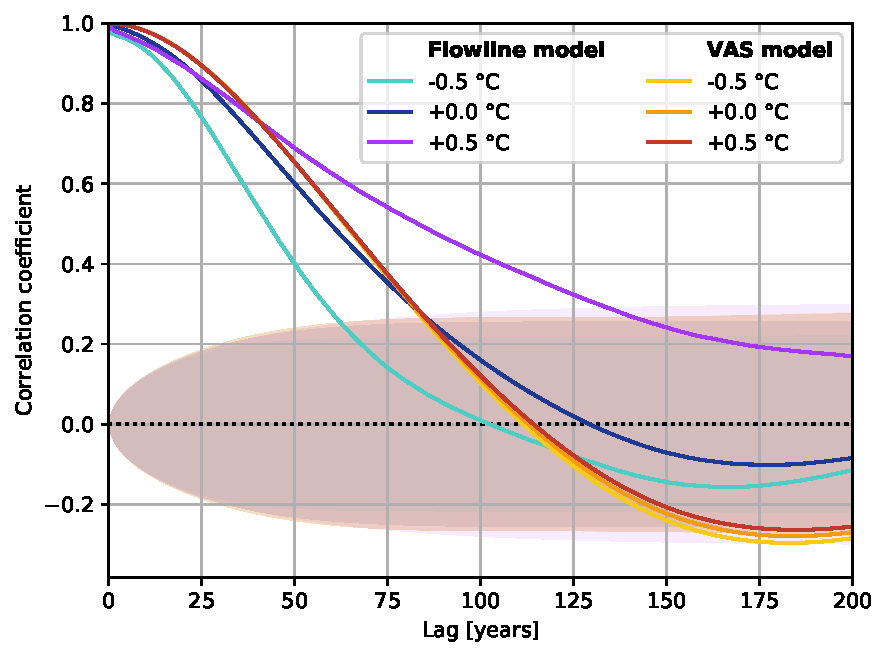
\includegraphics[width=\textwidth]{../plots/final_plots/acf/Findelgletscher.pdf}
        % \end{subfigure}

        \caption{Autocorrelation function of modeled length for lag times between zero and 200 years. Different lines represent different combinations of evolution model and climate scenario.
        The random climate scenario is based on an equilibrium climate, with different temperature biases.
        Cyan, blue and purple lines represent the flowline model, while yellow, orange and red lines represent the \vas{} model, with a temperature bias of \SI{-.5}{\celsius}, \SI{0}{\celsius} and \SI{+.5}{\celsius}, respectively.
        The \SI{99}{\percent} confidence intervals are shaded in the corresponding colors.}
        \label{fig:acf}
      \end{figure}
    
    % subsection sub:autocorrelation_analysis_results (end)

% section equilibrium_experiments (end)

% ==== SECTION 2 ===============================================================
\section{Sensitivity experiments} % (fold)
\label{sec:sensitivity_experiments_results}

% section sensitivity_experiments (end)

% ==== SECTION 3 ===============================================================
\section{Future projection} % (fold)
\label{sec:future_projection_results}

% section future_projection (end)